\chapter{Ionización de moléculas biológicas}

\section{Introducción}

El interés sobre el estudio de la ionización de moléculas biológicas por 
el impacto de iones de carga múltiple ha crecido en el último tiempo 
debido a sus aplicaciones~\cite{Liamsuwan:13}, que incluyen tratamientos 
médicos~\cite{Mohamad:17,Baskar:12,Denifl:11,Solov:09} y reconocimiento 
de contaminantes en materiales biológicos~\cite{Gafur:18,FerrazDias:13}. 
Particularmente, el estudio del daño causado por projectiles pesados 
cargados en blancos biológicos es relevante debido a su aplicación en la 
terapia contra el cáncer, que implementa haces de iones~\cite{Baskar:12}. 
La ionización de moléculas biológicas por iones cargados constituye el 
principal mecanismo de daño celular. Así, la efectividad de la radiación 
depende de la elección de los iones a implementar. En particular, 
estudios teóricos y experimentales con diferentes projectiles han 
concluido que los iones cargados de carbón podrían ser los iones más 
apropiados para dicha implementación~\cite{Mohamad:17}. Sin embargo, el 
estudio de tales sistemas representa un gran desafío desde el punto de 
vista teórico. 

A lo largo de las últimas décadas se ha propuesto una amplia variedad de 
métodos teóricos con el fin de predecir la ionización de estos sistemas 
colisionales. Por ejemplo, se ha estudiado la ionización de agua, bases 
del ADN y ARN debido al impacto de protones y partículas $\alpha$ 
implementando el método de trayectorias clásicas Monte Carlo~(\acs{ctmc}) 
en combinación con el criterio de sobrebarrera clásica~(\acs{cob}) 
\cite{Abbas:08,Lekadir:09}. Los primeros cálculos mecanico-cuánticos de 
este proceso en moléculas biológicas fueron realizados bajo el formalismo 
de la primera aproximación de Born~(\acs{fba})~\cite{DalCappello:08,
Champion:10}. A altas energías, este método perturbativo garantiza las 
leyes de $Z^2$, donde $Z$ es la carga del projectil incidente. Sin 
embargo, el daño causado por la ionización está concentrado en los 
alrededores del pico de Bragg, esto es, a energías de unos cientos de 
keV/amu. Sin embargo, es precisamente en esta región donde la FBA empieza 
a fallar. 

Una de las grandes dificultades del modelado de la ionización de estos 
sistemas está dada por está la descripción de la estructura del blanco
mediante métodos de primeros principios. Los primeros cálculos de las 
funciones de onda moleculares implementaron el método de Hartree--Fock
(\acs{hf}) con geometría optimizada, mediante la expansión de un centro 
(\acs{sce})~\cite{DalCappello:08} y el método de omisión completa de 
superposición diferencial (\acs{cndo})~\cite{Champion:10}. En este último 
trabajo, la hipótesis principal se basa en el modelo de átomo 
independiente~(\acs{iam}); así, las secciones eficaces moleculares de 
ionización se obtienen a partir de la combinación lineal de secciones 
eficaces atómicas pesadas, donde los factores de peso son obtenidos 
mediante el análisis de la población de los orbitales moleculares. 

Las limitaciones de los métodos perturbativos de primer orden son 
superadas implementando aproximaciones con correcciones de mayor orden. 
Por ejemplo, el trabajo de Galassi \textit{et al.} \cite{Galassi:00} 
predice con éxito la ionización de moléculas simples por impacto de 
protones mediante el método de onda continua distorsionada con estado 
inicial de Eikonal (\acs{cdw-eis}) \cite{Fainstein:88,Miraglia:08,
Miraglia:09}. Esta metodología también ha sido utilizada para modelar la 
ionización de nucleobases debido al impacto de protones~\cite{Galassi:12}.
%%%% Acá va la descripción de trabajo de Ludde et al. %%%%
Más recientemente, y también siguiendo la línea del \acs{iam}, Lu\"udde 
y colaboradores~\cite{Ludde:16,Ludde:18,Ludde:19,Ludde:20} han propuesto 
la combinación de secciones eficaces atómicas con correcciones 
geométricas de apantallamiento. En este caso, los autores obtienen las 
secciones eficaces atómicas a partir de la teoría del functional densidad 
dependiente del tiempo~(\acs{tddft}). 

En este capítulo trataremos los dos aspectos principales de la ionización 
de moléculas biológicas debido a iones de carga múltiple: el orden de 
aproximación del proceso colisional ion--molécula y el método usado para 
describir el blanco. El modelo propuesto aquí para tratar la ionización 
de blancos moleculares por iones cargados implementa el IAM, que se 
desprende de la regla aditiva de Bragg~(\acs{bar}). De manera que, 
primeramente, se implementará el método CDW-EIS para obtener una 
descripción apropiada del mecanismo de daño principal causado por los 
átomos que constituyen las moléculas a estudiar. Por simplicidad, de aquí 
en adelante la aproximación CDW-EIS será referida como CDW. Detalles 
sobre el método y los cálculos realizados se presentan en la 
Sección~\ref{sec:atoms}. Nuestro trabajo se desarrolla bajo la premisa de 
que el proceso de ionización es el mecanismo que deposita la mayor 
cantidad de energía primaria en el sistema. Sin embargo, se conoce que 
los electrones residuales de la ionización son una fuente significativa 
de daño biológico local~\cite{Denifl:11}. En efecto, los electrones 
secundarios son incluidos en simulaciones de Monte 
Carlo~\cite{Champion:16,Quinto:17,Acocer-Avila:19}, y por lo tanto su 
comportamiento requiere especial atención. En las 
Secciones~\ref{subsec:meanener} y \ref{subsec:meanang}, estudiamos las 
distribuciones energéticas y angulares medias de los electrones ejectados 
de los blancos atómicos según el método CDW. Contrariamente a lo predicho 
por la FBA, encontramos una dependencia sustancial de estos valores con 
la carga del projectil. En la Sección~\ref{sec:SSM}, tratamos la 
complejidad de la ionización molecular implementando el modelo 
estequiométrico simple (\acs{ssm}), el cual consiste en asumir que las 
moleculas están compuestas por átomos aislados e independientes, y que la 
sección eficaz total se expresa como una combinación lineal de cálculos 
atómicos pesados según la estequiometría de la molécula. Así, 
implementando en conjunto el método CDW y SSM, obtenemos secciones 
eficaces de ionización de diversas moléculas de interés biológico, 
incluyendo las cinco nucleobases --adenina, citosina, guanina, timina, 
uracilo--, tetrahidrofurano (\acs{thf}), pirimidina y agua, debido al 
impacto de antiprotones, H$^{+}$, He$^{2+}$, Be$^{4+}$, C$^{6+}$, y 
O$^{8+}$. 

En la Sección~\ref{sec:scaling}, estudiamos diversas reglas de escala. 
Por ejemplo, examinamos la regla de escala de Toburen~\cite{Toburen:75,
Toburen:76}, que establece que la razón entre la sección eficaz de 
ionización y el número de electrones débilmente ligados se puede ubicar 
sobre una delgada banda universal en términos de la velocidad del 
projectil. Aplicamos esta regla a un número significativo de sistemas 
colisionales, incluyendo --además de los blancos ya mencionados-- 
hidrocarburos y moléculas CHNO. Encontramos que la implementación de la 
ley de escala no es satisfactoria en los resultados SSM--CDW. Sin 
embargo, a partir del estudio de las secciones eficaces atómicas CDW, el 
ancho de las bandas resultantes, correspondientes a cada ion, puede ser 
reducido significativamente optimizando los números de electrones activos 
de cada átomo constituyente. Así, se proponen un nuevo conjunto de 
electrones débilmente ligados en diversos sistemas moleculares. La regla 
de escala resultante es implementada a nuestros valores teóricos y 
comparada con datos experimentales disponibles. Por otro lado, siguiendo 
la escala propuesta por Montenegro y colaboradores~\cite{Dubois:13,
Montenegro:13}, la ley de escala $Z^2$ se reescribe en términos de un 
parámetro $\alpha$. Combinando el escaleo de las secciones eficaces 
totales con el número de electrones activos de los blancos y la carga del 
ion incidente, obtenemos una regla de escala única e independiente del 
sistema colisional. La generalidad de nuestra regla es puesta a prueba 
con datos experimentales de otros sistemas colisionales, no considerados 
previamente en esta investigación.

Por último, la aproximación SSM propuesta considera los átomos en la 
molécula como si fueran neutrales, lo cual no es correcto. En la 
Sección~\ref{sec:molcalculations}, consideramos los cálculos de 
estructura molecular realizados con el código {\sc gamess}~\cite{gamess} 
para computar el exceso o defecto de densidad electrónica en los átomos 
que componen las moléculas. Así, proponemos una fórmula estequimétrica 
modificada para tener en cuenta el alejamiento de la neutralidad de los 
átomos. Encontramos que modificación a la aproximación SSM para las 
moléculas de ADN no introduce cambios sustanciales en las secciones 
eficaces totales de ionización.

%%%%%%%%%%%%%%%%%%%%%%%%%%%%%%%%%%%%%%%%%%%%%%%%%%%%%%%%%%%%%%%%%%%%%%%%
\section{Ionización de átomos constituyentes}
\label{sec:atoms}
%%%%%%%%%%%%%%%%%%%%%%%%%%%%%%%%%%%%%%%%%%%%%%%%%%%%%%%%%%%%%%%%%%%%%%%%

La sección de ionización total $\sigma_{\alpha}$ del átomo $\alpha$, que 
será luego implementada en el modelo molecular, se obtiene a partir de la 
aproximación del método CDW (ver Apéndice~\ref{app:CDW}). Las 
funciones de onda radiales de los estados inicial ligado y final continuo 
se calculan usando el código~\textsc{radialf}, desarrollado por Salvat y 
colaboradores~\cite{salvat1995}, e implementando potenciales efectivos. 
Los potenciales utilizados se obtuvieron a partir de la implementación 
del método de Inversión Depurada (\acs{dim})~\cite{Mendez:16,Mendez:18} 
desarrollado en el capítulo anterior. Usamos un par de miles de puntos 
como pivotes para resolver la ecuación de Schr\"{o}dinger, dependiendo 
del número de oscilaciones del estado del contínuo. La integración radial 
fue realizada usando la técnica de interpolación cúbica. Las funciones de 
onda del estado final en el continuo fueron expandidas como
\begin{equation}
\psi_{\mbox{\scriptsize$\mathbf{k}$}}^-(\mathbf{r})=\sum_{l=0}^{l_{\max
}}\sum_{m=-l}^l R_{kl}^-(r)\,Y_l^m(\hat{r})\,Y_l^{m^*}
(\hat{k})\,.
\label{eq:contwave}
\end{equation}
El número de momentos angulares $l$ considerados variaron desde 8, para 
electrones expulsados a muy bajas energías, hasta $l_{\max}\sim 30$, para 
las energías más altas consideradas. Se requirieron el mismo número de 
ángulos azimutales para obtener las secciones eficaces diferenciales 
cuádruples. 
%El cálculo realizado no muestra discrepancias en las versiones 
%posteriores y previas del método. 
Cada sección eficaz atómica total fue calculada usando entre 35 y 100 
valores de transferencia de momento, 28 ángulos electrónicos fijos, y 
alrededor de 45 valores de energía electrónica, dependiendo de la energía 
de impacto del proyectil. Para más detalle sobre la metodología, se puede 
consultar el trabajo de la Ref.~\cite{Montanari:17-iongasesnobles}. 

\begin{figure}
\centering
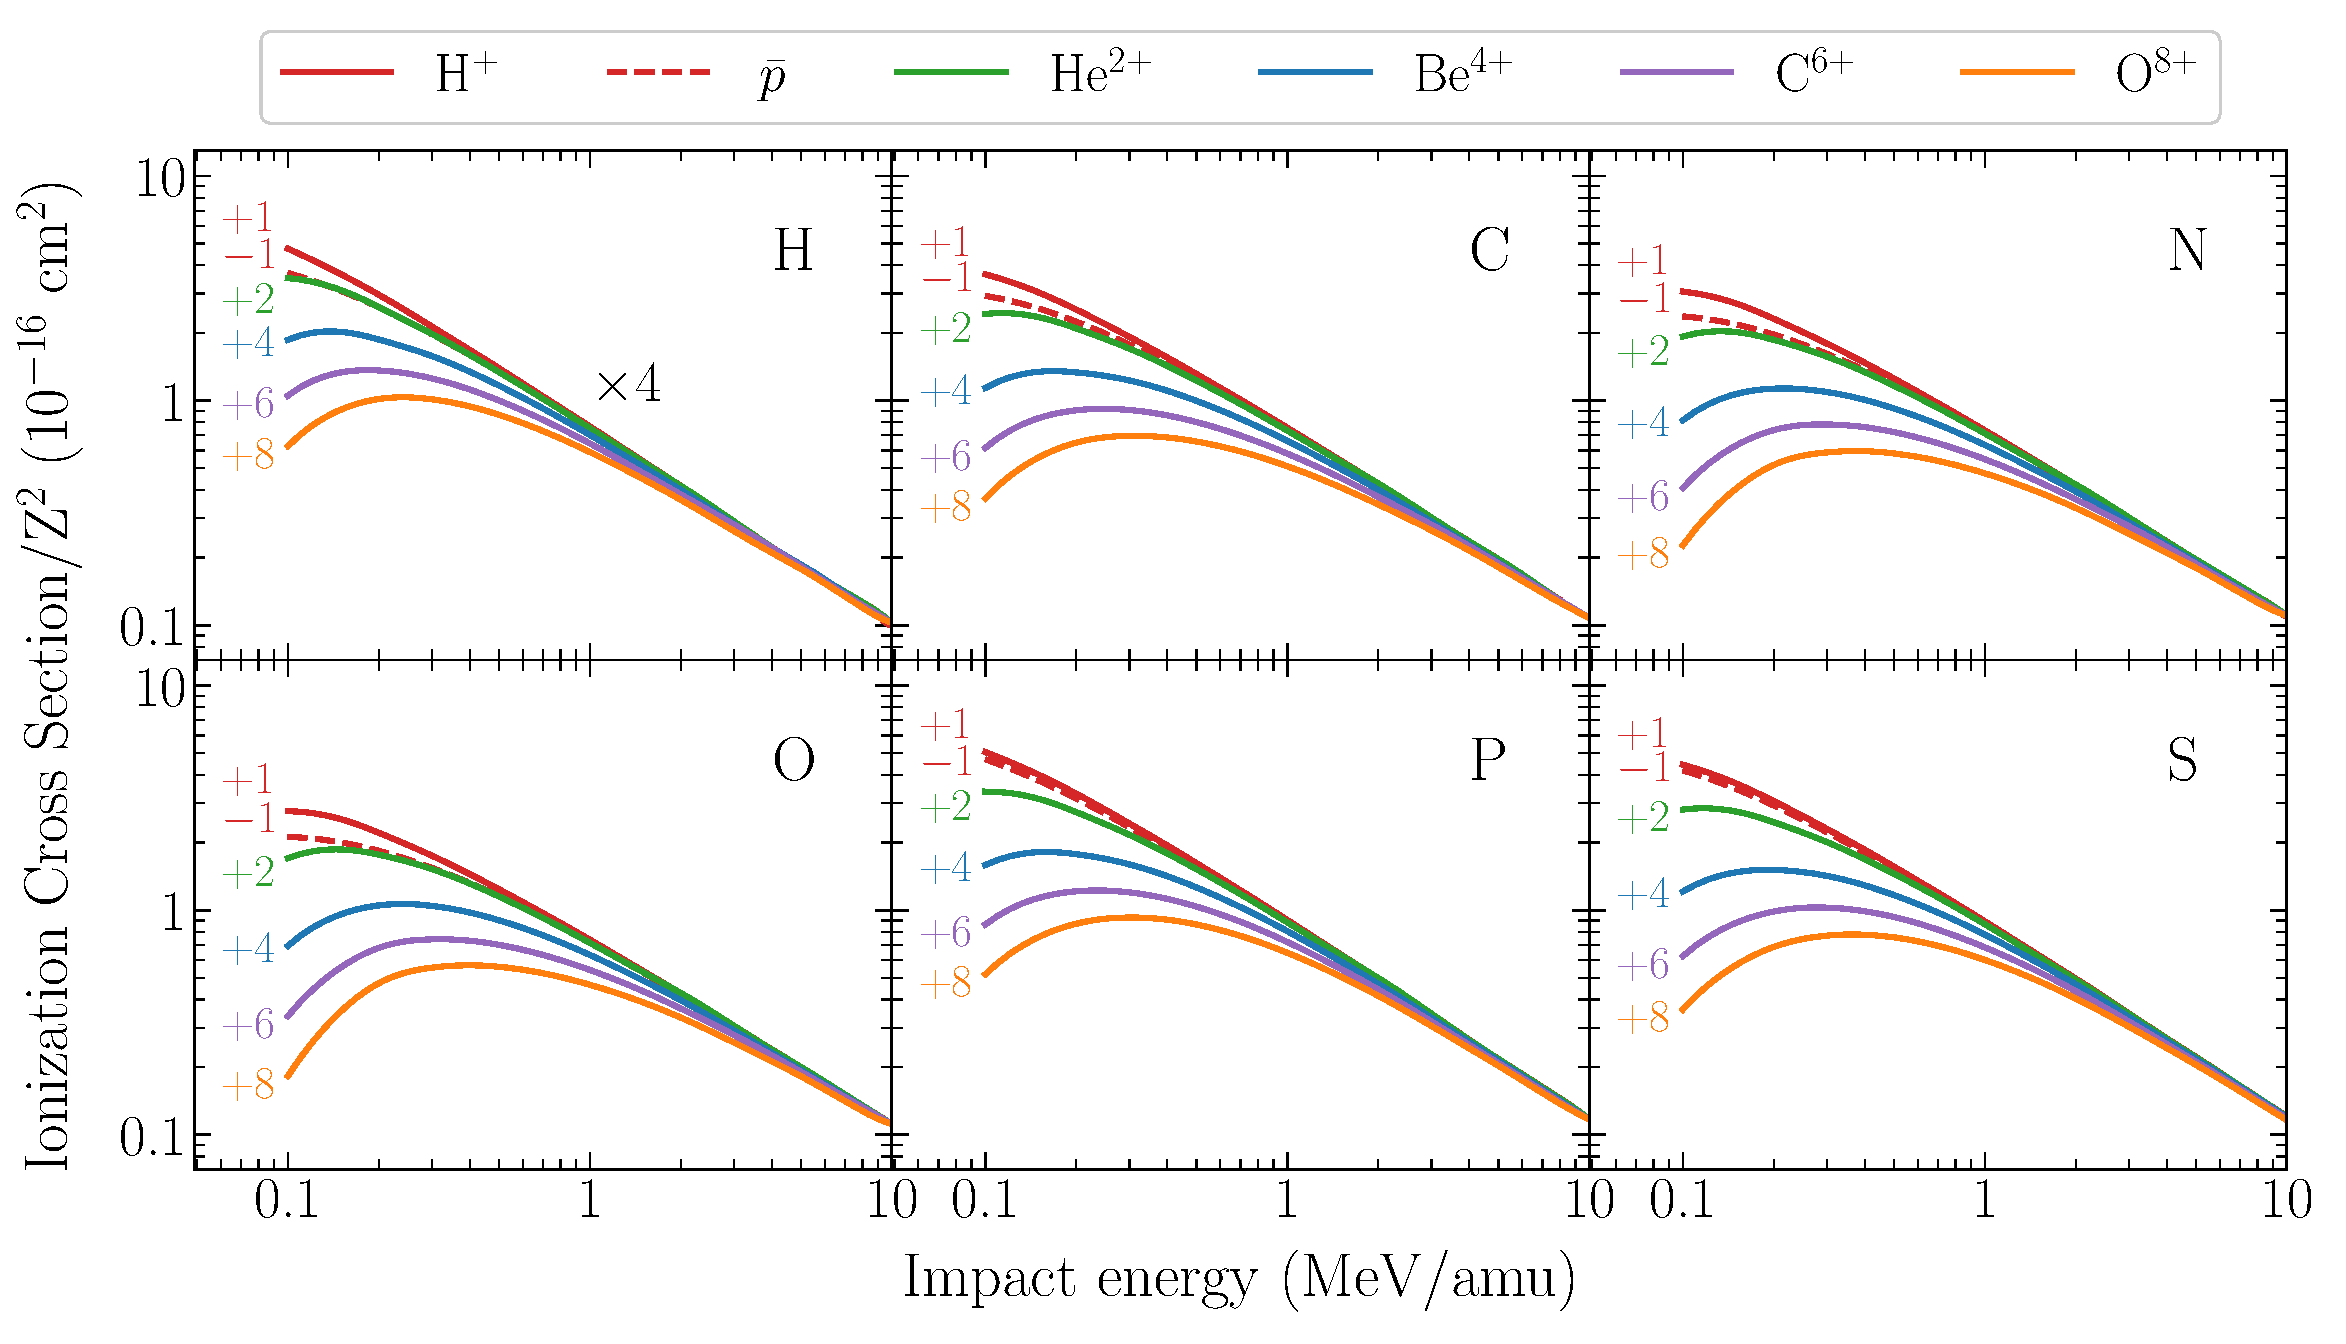
\includegraphics[width=0.9\textwidth]{ionmol/atomicscaling.eps}
\caption[Sección eficaz total de ionización atómica CDW reducida.]
{Sección eficaz total de ionización CDW reducida $\sigma_{\alpha}/Z^2$ 
de cuatro blancos atómicos relevantes. Curvas: cálculos teóricos CDW. 
Símbolos: ionización de H por impacto de H$^+$~\cite{Shah:81}; ionización 
por impacto de $e^-$ en H~\cite{Shah:87}, C~\cite{Brook:78}, 
N~\cite{Brook:78} y O~\cite{Thompson:95}.}
\label{fig:atomscaling}
\end{figure} 

La mayor parte de las moléculas orgánicas contienen átomos de hidrógeno, 
carbono, nitrógeno, oxígeno, fósforo y azufre. Los sistemas colisionales
que estudiamos a continuación están compuestos por cuatro blancos 
atómicos, $\alpha=$ H, C, N, O, y sies proyectiles incidentes: 
antiprotones $\bar{p}$, H$^{+}$, He$^{2+}$, Be$^{4+}$, C$^{6+}$, y 
O$^{8+}$. En la Fig.~\ref{fig:atomscaling} se muestran las secciones 
eficaces totales de ionización de los 24 sistemas blanco--proyectil 
resultantes usando el método CDW. Para comparar los resultados 
correspondiente a cada sistema colisional en una única figura, 
consideramos el hecho que en la primera aproximación de Born, la sección 
eficaz de ionización escala con el cuadrado de la carga del ion 
incidente, es decir $Z^{2}$. Las energías de impacto consideradas van de 
$0.1$ a 10 MeV/amu, donde el método CDW tiene validez. Particularmente, 
para los proyectiles de carga más altas, el valor de energía mínimo donde 
se espera que la CDW tenga validez aumenta hasta aproximadamente 400~keV. 
Nuestros resultados se comparan con secciones eficaces experimentales 
para el caso de ionización de H por impacto de H$^+$~\cite{Shah:81}. Se 
incluyen mediciones de ionización por impacto de electrones en 
H~\cite{Shah:87}, C~\cite{Brook:78}, N~\cite{Brook:78} y 
O~\cite{Thompson:95}, con la correspondiente conversión de equivelocidad, 
para energías incidentes superiores a 300~eV. Es esperable que en esta 
región de energía la ionización por impacto de H$^+$ y $e^-$ convergen. 
También realizamos cálculos similares con la FBA (no se muestran aquí), 
y corroboramos que ésta provee resultados confiables para valores de 
energía mayores a unos cuantos MeV/amu. Para nuestros resultados teóricos,
usamos el mismo color de línea para indicar la carga del proyectil en 
todas las figuras que se muestran a lo largo de este Capítulo: 
discontinua--roja, sólida--roja, azul, magenta, oliva y naranja para 
antiprotones, H$^{+}$, He$^{2+}$, Be$^{4+}$, C$^{6+}$, y O$^{8+}$, 
respectivamente. En el caso de los datos experimentales, se usan símbolos 
de los mismos colores para denotar la carga del ion incidente 
correspondiente. Los resultados de ionización de cada capa se pueden 
hallar en la Ref.~\cite{Miraglia:19}.

%%%%%%%%%%%%%%%%%%%%%%%%%%%%%%%%%%%%%%%%%%%%%%%%%%%%%%%%%%%%%%%%%%%%%%%%
\subsection{Distribución energética de electrones}
\label{subsec:meanener}
%%%%%%%%%%%%%%%%%%%%%%%%%%%%%%%%%%%%%%%%%%%%%%%%%%%%%%%%%%%%%%%%%%%%%%%%

En un medio biológico dado, la ionización directa debido al impacto de un 
ion representa solo una fracción del daño total. Los electrones 
secundarios, así como el retroceso de los iones del blanco, también 
contribuyen sustancialmente al daño total~\cite{Denifl:11}. Podemos 
considerar que la sección eficaz de ionización diferencial en función de 
la energía del electrón eyectado $E$ de la capa $nl$ del átomo $\alpha$,
$d\sigma_{\alpha nl}/dE$, es una función de distribución simple~\cite{Surdutovic:18}. Así, siguiente a Abril y 
coloboradores~\cite{Abril:15}, definimos un valor medio 
$\overline{E}_{\alpha}$, 
\begin{eqnarray}
\overline{E}_{\alpha} &=&\frac{\langle E_{\alpha}\rangle}{\langle
1\rangle}=\frac{1}{\sigma_{\alpha}}\sum\limits_{nl}\int dE\,E
\frac{d\sigma_{\alpha,nl}}{dE}\,,  
\label{eq:meanener} \\
\langle 1\rangle &=&\sigma_{\alpha}=\sum\limits_{nl}\int dE\,
\frac{d\sigma_{\alpha,nl}}{dE}\,. 
\label{eq:normener}
\end{eqnarray}
donde $\Sigma_{nl}$ tiene en cuenta la suma de las diferentes 
contribuciones de cada capa del elemento $\alpha$.

\begin{figure}
\centering
\includegraphics[width=0.9\textwidth]{ionmol/ener_mean.eps}
\caption[Distribución energética media de electrones emitidos.]
{Distribución energética media de electrones emitidos por la ionización 
debido al impacto de iones cargados dada por la Ec.~(\ref{eq:meanener}). 
Curvas: cálculos teóricos FBA con $Z=1$ (punteada) y CDW (sólidas y 
discontinua).}
\label{fig:emittedener}
\end{figure} 

Las energías medias de los electrones emitidos $\overline{E}_{\alpha}$ 
por H, C, N y O se muestran en la Fig.~\ref{fig:emittedener}. El rango 
de velocidad de impacto fue reducido a $v=10$~a.u. debido a las 
limitaciones numéricas en la expansión de esféricos armónicos dados por 
la Ec.~(\ref{eq:contwave}). A medida que la velocidad de impacto $v$ 
aumenta, también aumenta $\langle E_{\alpha}\rangle$ y $l_{\max}$, lo que 
resulta en la inclusión de funciones con muchas oscilaciones en el 
integrando. Más aún, el integrando de $\langle E_{\alpha}\rangle$ incluye 
la energía cinética $E$, que reduce su valor en la región de energías 
pequeñas y lo incrementa para valores grandes, haciendo que el resultado 
sea más sensible a los momentos angulares mayores. Independientemente, 
para $v>10$ a.u., la primera aproximación de Born es válida. 

En la Fig.~\ref{fig:emittedener} estimamos el valor de 
$\overline{E}_{\alpha}$ de los electrones emitidos en el rango de energía 
de 10 a 70 eV, para todos los blancos atómicos. Nuestros resultados 
concuerdan con los hallazgos experimentales~\cite{Surdutovic:18}. Como se 
puede observar en la figura, el valor de energía media es 
sorprendentemente sensible a la carga del proyectil $Z$, que puede 
duplicar los resultados de protón en la región intermedia, i.e., 
100--400 keV/amu. El efecto observado puede atribuirse al repulsión 
electrónica causada por los iones de carga múltiple en los electrones de 
baja energía. Este comportamiento no se puede encontrar en la primera 
aproximación de Born, donde la ley de escala $Z^2$ cancela la dependencia 
con $Z$ de la Ec.~(\ref{eq:meanener}). A altas energías, 
$\overline{E}_{\alpha}$ tiende a un valor universal para todos los iones, 
como puede verse en la Fig.~\ref{fig:emittedener}.

%%%%%%%%%%%%%%%%%%%%%%%%%%%%%%%%%%%%%%%%%%%%%%%%%%%%%%%%%%%%%%%%%%%%%%%%
\subsection{Distribución angular de electrones}
\label{subsec:meanang}
%%%%%%%%%%%%%%%%%%%%%%%%%%%%%%%%%%%%%%%%%%%%%%%%%%%%%%%%%%%%%%%%%%%%%%%%

\begin{figure}
\centering
\includegraphics[width=0.9\textwidth]{ionmol/ang_mean.eps}
\caption[Distribución angular media de electrones emitidos.]
{Distribución angular media de electrones emitidos por la ionización 
debido al impacto de iones cargados dada por Ec.~(\ref{eq:meanang}). 
Curvas: cálculos teóricos FBA con $Z=1$ (punteada) y CDW (sólidas y 
discontinua).}
\label{fig:emittedang}
\end{figure} 

Como mencionamos anteriormente, la emisión de electrones secundarios 
contribuye al daño total. Entonces, no sólo es esencial conocer la 
distribución de energía de los electrones eyectados, sino también la 
dirección a la que éstos son emitidos. Una vez más, podemos considerar 
que la sección eficaz diferencial de ionización es función del ángulo 
sólido de eyección del electrón $\Omega$, $d\sigma_{\alpha,nl}/d\Omega$, 
y puede expresarse como una función de distribución. Así, el ángulo medio 
de emisión $\overline{\theta}_{\alpha}$ se define como
\begin{eqnarray}
\overline{\theta}_{\alpha}&=&\frac{\langle\theta_{\alpha}\rangle}
{\langle 1\rangle}=\frac{1}{\sigma_{\alpha}}\sum\limits_{nl}
\int d\Omega\,\theta\,\frac{d\sigma_{\alpha,nl}}{d\Omega} 
\label{eq:meanang} \\
\langle 1\rangle &=&\sigma_{\alpha}=\sum\limits_{nl}\int d\Omega\,
\frac{d\sigma_{\alpha,nl}}{d\Omega}\,.
\end{eqnarray}

Los ángulos medios de emisión electrónica $\overline{\theta}_{\alpha}$ 
de los cuatro átomos y seis iones estudiados en esta sección se muestran 
en la Fig.~\ref{fig:emittedang}. Se puede observar una dependencia 
significativa de $\overline{\theta}_{\alpha}$ con $Z$ para todos los 
sistemas colisionales. Una vez más, este efecto no puede ser observado en 
la implementación del FBA (línea punteada).

En la emisión de electrones de baja energía, la dispersión angular es 
casi isotrópica~\cite{Rudd:92}. Un valor típico para el ángulo de 
eyección considerado en la literatura es 
$\overline{\theta}_{\alpha}\sim$~70\textdegree~\cite{Surdutovic:18}, el 
cual resulta bastante certero en el rango de validez de la FBA para 
cualquier blanco. Sin embargo, cuando se usa la aproximación de onda 
distorsionada, $\overline{\theta}_{\alpha}$ disminuye sustancialmente con 
$Z$ en la región de energía intermedia, como se observa en la 
Fig.~\ref{fig:emittedang}. Cuanto mayor sea la carga $Z$, menor será 
$\overline{\theta}$. Por supuesto, este efecto solo es válido en energías 
intermedias y no en el rango de altas energías.

Para ilustrar esta característica, consideramos el impacto de C$^{6+}$ 
con una energía de 500~keV sobre oxígeno. La primera aproximación de Born 
predice electrones emitidos con energías medias de $46.7$ eV y ángulos 
medios de 78\textdegree, mientras que la aproximación CDW establece 
energías medias de $62.5$~eV y un ángulo de emisión igual a 60\textdegree. 
Nuestros resultados sugieren una penetración más profunda de los 
electrones secundarios con una orientación más cercana a la dirección del 
ion. Podemos atribuir esta corrección de la dirección de avance al efecto 
de captura del continuo.

Además, la Fig.~\ref{fig:emittedang} proporciona una descripción 
ilustrativa del comportamiento de los antiprotones: el proyectil repele 
los electrones, siendo $\overline{\theta}_{\alpha}\sim$~90\textdegree. 
Nótese el descripción opuesta de protones y antiprotones dada por la CDW 
con respecto a la primera aproximación de Born; este fenómeno constituye 
un efecto Barkas angular.

%%%%%%%%%%%%%%%%%%%%%%%%%%%%%%%%%%%%%%%%%%%%%%%%%%%%%%%%%%%%%%%%%%%%%%%%
\section{El modelo estequiométrico}
\label{sec:SSM}
%%%%%%%%%%%%%%%%%%%%%%%%%%%%%%%%%%%%%%%%%%%%%%%%%%%%%%%%%%%%%%%%%%%%%%%%

El modelo estequiométrico simple (\acs{ssm}) que proponemos aquí para 
predecir secciones eficaces moleculares totales de ionización está basado 
en la aproximación de átomo independiente, también llamada regla aditiva 
de Bragg. Este modelo supone que los átomos que componen una molécula $M$ 
interactúan con el proyectil incidente pero no entre sí. Así, si 
suponemos que la molécula $M$ está compuesta por $n_{\alpha}$ átomos del 
elemento $\alpha$, el modelo estequiométrico aproxima la sección eficaz 
total de ionización de la molécula $\sigma_M$ como la suma de secciones 
eficaces totales de ionización de los átomos aislados $\sigma_{\alpha}$ 
ponderada por $n_{\alpha}$, 
\begin{equation}
\sigma_{M}=\sum\limits_{\alpha}n_{\alpha}\sigma_{\alpha}\,.  
\label{eq:sumion}
\end{equation}
Los blancos moleculares examinados a lo largo de este capítulo se 
clasifican en tres familias: CH, CHNO, y ADN, como se muestra en la 
Tabla~\ref{tab:families}.

\begin{table}
\begin{center}
\begin{tabular}{|p{0.08\textwidth}|p{0.8\textwidth}|}
\hline
\multirow{2}{*}{CH} & CH$_4$ (metano), C$_2$H$_2$ (acetileno), 
C$_2$H$_4$ (eteno), C$_2$H$_6$ (etano), \\ & C$_6$H$_6$ (benceno) \\
\hline
\multirow{2}{*}{CHNO} & C$_5$H$_5$N (piridina), C$_4$H$_4$N$_2$ (pirimidina), 
C$_2$H$_7$N (dimetilamina), \\ & CH$_5$N (monometilamina), 
C$_4$H$_8$O (THF) \\[0.2em]
\hline
\multirow{2}{*}{DNA} & C$_5$H$_5$N$_5$ (adenina), C$_4$H$_5$N$_3$O (citosina), 
C$_5$H$_5$N$_5$O (guanina), \\ & C$_5$H$_6$N$_2$O$_2$ (timina),
C$_4$H$_4$N$_2$O$_2$ (uracilo), H$_2$O (agua) \\
\hline
\end{tabular}
\caption[Blancos moleculares examinados y clasificados en tres familias.]
{Blancos moleculares de interés examinados en el presente trabajo y 
clasificados en tres familias.}
\label{tab:families}
\end{center}
\end{table}

En la Fig.~\ref{fig:crossDNA_1} reportamos las secciones eficaces de 
ionización totales reducidas con la carga del ión incidente, 
$\sigma_M/Z^2$, de las nucleobases del ADN --adenina, citosina, guanina y 
timina-- debido al impacto de iones de carga múltiple, que se obtienen a 
partir de la aproximación SSM y el método CDW. Para adenina, los datos 
experimentales disponibles para el impacto de protones~\cite{Iriki:11} 
tienen un excelente acuerdo con nuestras 
predicciones. La medición de C$^{4+}$~\cite{Sens:20} sobre adenina 
coincide con el modelo SSM--CDW dentro del margen de error. Si bien esta
data es preliminar, la comparación es alentadora en cuanto a la respuesta 
de nuestro modelo para la ionización de projectiles de carga múltiple. 
Por otro lado, los resultados teóricos de ionización de adenina debido a 
C$^{6+}$ discrepan con el valor experimental 
disponible~\cite{Bhattacharjee:19} en un factor dos. Esta discrepancia es 
intrigante ya que la medición se encuentra en el rango de altas energías, 
donde generalmente la teoría predice muy bien los experimentos.

No hemos encontrado en la bibliografía datos experimentales de ionización 
por impacto de iones cargados para el resto de las nucleobases de ADN.
Incluimos en la Fig.~\ref{fig:crossDNA_1} mediciones de ionización por 
impacto de electrones~\cite{Rahman:16}, con la correspondiente 
conversión de equivelocidad, para energías incidentes superiores a 
300~eV. En esta región, la sección eficaz de ionización por impacto de 
protones y electrones debería coincidir. Aunque las mediciones de impacto 
de electrones están por encima de nuestros hallazgos para todos los 
objetivos moleculares, vale la pena señalar que los resultados SSM--CDW
concuerdan muy bien con otras predicciones teóricas de ionización por 
impacto de electrones~\cite{mozejko2003,tan2018}.

\begin{figure}
\centering
\includegraphics[width=0.9\textwidth]{ionmol/adn1.eps}
\caption[Sección eficaz total de ionización reducida por $Z$ (Parte I).]
{Sección eficaz total de ionización CDW reducida $\sigma_{M}/Z^2$ como 
una función de la energía de impacto del ion. Símbolos: datos 
experimentales de impacto de protón~\cite{Iriki:11}, 
C$^{4+}$~\cite{Sens:20}, C$^{6+}$~\cite{Bhattacharjee:19}, y 
e$^-$~\cite{Rahman:16} con conversión de equivelocidad.}
\label{fig:crossDNA_1}
\end{figure} 

\begin{figure}
\centering
\includegraphics[width=0.9\textwidth]{ionmol/adn2.eps}
\caption[Sección eficaz total de ionización reducida por $Z$ (Parte II).]
{Sección eficaz total de ionización CDW reducida $\sigma_{M}/Z^2$ como 
una función de la energía de impacto del ion. Símbolos: datos 
experimentales de impacto de protón en uracilo~\cite{itoh2013}, 
pirimidina~\cite{wolff2014}, THF~\cite{wang2016} y agua~\cite{Luna2007,
Bolorizadeh86,H_Rudd85,toburen80}. Impacto de C$^{4+}$~\cite{Sens:20} y 
C$^{4+}$, C$^{6+}$, O$^{6+}$, F$^{6+}$, O$^{8+}$, y F$^{8+}$ en 
uracilo~\cite{agnihotri2012,agnihotri2013}. Ionización de agua por 
impacto de He$^{2+}$~\cite{Ohsawa05,He_Rudd85,toburen80}, 
C$^{6+}$~\cite{DalCappello2009,Bhattacharjee:17} y 
O$^{8+}$~\cite{Bhattacharjee:16}. 
Impacto de e$^-$~\cite{bug2017,wolf2019,fuss2009} con conversión de 
equivelocidad.}
\label{fig:crossDNA_2}
\end{figure} 

Las secciones eficaces de ionización total reducidas $\sigma_M/Z^2$ 
para uracilo, pirimidina, THF y agua se muestran en la 
Fig.~\ref{fig:crossDNA_2}. En uracilo, las mediciones experimentales de 
ionización por impacto de protones de Itoh~\textit{et al.}~\cite{itoh2013} 
tienen un buen acuerdo con nuestras predicciones. Sin embargo, para el 
mismo blanco, nuestra teoría predice secciones eficaces con un factor 
dos por encima de las mediciones experimentales de Agnihotri 
\textit{et al.}~\cite{agnihotri2012,agnihotri2013} para el impacto de 
iones de carga múltiple. No obstante, cabe señalar que nuestros 
resultados teóricos coinciden con los cálculos de Champion, Rivarola y 
colaboradores~\cite{agnihotri2012,champion2012}. Los cálculos recientes 
de Sarkadi~\cite{sarkadi2016} empleando el método CTMC también se 
encuentran por arriba de los valores experimentales de Tribedi y 
colaboradores~\cite{agnihotri2012,agnihotri2013}. Además, hemos incluimos 
una reciente medición experimental preliminar de Sens y 
colaboradores~\cite{Sens:20} para la ionización en uracilo debido al 
impacto de C$^{4+}$ que coincide con la teoría, lo que podría indicar 
algún problema con los valores experimentales de Agnihotri y 
colaboradores. 

Para pirimidina, mostramos una comparación de nuestros resultados con los 
datos experimentales de ionización por impacto de protones de Wolff
\textit{et al.}~\cite{wolff2014} y también para la ionización por impacto 
de electrones~\cite{bug2017} a altas energías. Las mediciones de impacto 
de electrones concuerdan con las predicciones SSM--CDW para energías 
superiores a 500~keV. Inesperadamente, las secciones eficaces de 
ionización por impacto de protones son significativamente más bajas que 
nuestros resultados. Una mayor cantidad de experimentos se encuentran 
disponibles para la ionización de la molécula de THF por impacto de 
H$^+$~\cite{wang2016} y de e$^-$~\cite{bug2017,wolf2019,fuss2009}. Los 
resultados que obtenemos de la combinación del SSM y las secciones 
eficaces atómicas CDW muestran un buen acuerdo general con esta data.

En el caso de la molécula de agua, los resultados experimentales son más 
abundantes que para el resto de los blancos. Los resultados 
experimentales~\cite{Luna2007,Bolorizadeh86,H_Rudd85,Ohsawa05,He_Rudd85,
toburen80,Bhattacharjee:16} coinciden con nuestras predicciones para 
todos los iones de carga múltiple examinados aquí, excepto para 
C$^{6+}$~\cite{DalCappello:09,Bhattacharjee:17}, donde la teoría 
sobrestima la ionización en un factor dos en el rango de altas energías. 
A diferencia de las nucleobases, pirimidina y THF, la estequiometría del 
agua es más simple; sin embargo, observamos que nuestro modelo responde 
bien incluso para predecir la ionización de moléculas pequeñas debido a 
la incidencia de iones pesados, tal como es el caso de O$^{6+}$.

%%%%%%%%%%%%%%%%%%%%%%%%%%%%%%%%%%%%%%%%%%%%%%%%%%%%%%%%%%%%%%%%%%%%%%%%
\section{Reglas de escala}
\label{sec:scaling}

%%%%%%%%%%%%%%%%%%%%%%%%%%%%%%%%%%%%%%%%%%%%%%%%%%%%%%%%%%%%%%%%%%%%%%%%
\subsection{Escala con electrones activos del blanco}
\label{subsec:ne_scaling}

%%%%%%%%%%%%%%%%%%%%%%%%%%%%%%%%%%%%%%%%%%%%%%%%%%%%%%%%%%%%%%%%%%%%%%%%
\subsubsection{Regla de Toburen}
\label{subsec:toburen}
%%%%%%%%%%%%%%%%%%%%%%%%%%%%%%%%%%%%%%%%%%%%%%%%%%%%%%%%%%%%%%%%%%%%%%%%

Toburen y colaboradores~\cite{Toburen:75,Toburen:76} propusieron el 
primer modelo fenomenológico completo y simple para la eyección de 
electrones de moléculas complejas. Los autores encontraron conveniente 
escalar la sección eficaz de ionización experimental en términos del 
número de electrones ligados débilmente, o activos, $n_e$. En general, 
este número está dado por la cantidad de electrones en la capa de 
valencia. Así, por ejemplo, para C, N y O, este número es igual al número 
total de electrones del átomo menos la capa K. 

Siguiendo a Toburen \textit{et al.}, definimos la sección eficaz de 
ionización escalada por el número de electrones débilmente ligado 
$\sigma_e$ para la molécula $M$ como
\begin{equation}
\sigma_e=\frac{\sigma_M}{n_e}\,, 
\label{eq:cross-ne} 
\end{equation}
donde $n_e=\sum_{\alpha}n_{\alpha}\nu_{\alpha}$ es el número total de 
electrones activos en el proceso colisional, y $\nu_{\alpha}$ es el 
número de electrones débilmente ligado en cada átomo $\alpha$. Para los 
blancos atómicos considerados aquí, los números de Toburen están dados 
por 
\begin{equation}
\nu_{\alpha}^T=\left\{ 
\begin{array}{ll}
1, & \text{para H,} \\
4, & \text{para C,} \\ 
5, & \text{para N,} \\ 
6, & \text{para O}\,.
\end{array}\right.
\label{eq:neToburen} 
\end{equation} 

La regla de Toburen se puede enunciar diciendo que $\sigma_{e}$ es un 
parámetro universal, que depende únicamente de la velocidad y naturaleza
del ion incidinte, aplicable en la región de $0.25$ a 5~MeV/amu. A 
muy altas energías, la probabilidad de ionizar electrones de la capa K 
es mayor. Así, en esta región, el número total de electrones activos 
será diferente. Una dependencia similar con el número de electrones 
ligados débilmente fue hallada por Itoh y coloboradores~\cite{itoh2013} 
para el impacto de protones sobre uracilo y adenina.

Siguiendo la ley de escala de Toburen, calculamos las secciones eficaces 
CDW escaladas con el número de electrones activos de Toburen, 
$\sigma_{e}^T$, para los blancos moleculares dados en la 
Tabla~\ref{tab:families}. Nuestros resultados se muestran en la 
Fig.~\ref{fig:newscaling}(a) en función de la energía de impacto para 
diferentes proyectiles de carga múltiple. Aunque la escala de Toburen se 
mantiene para altas energías, su desempeño no es muy satisfactorio: como 
se puede observar en la figura, la banda universal es bastante ancha.

\begin{figure}[t]
\centering
\includegraphics[width=0.9\textwidth]{ionmol/CDWscaling.eps}
\caption[Sección eficaz de ionización molecular escalada por $n_e$.]
{Sección eficaz de ionización molecular escalada por número de electrones 
débilmente ligados usando (a)~los números de Toburen $\nu_{\alpha}^T$, y 
(b) los números CDW $\nu_{\alpha}^{\text{CDW}}$ propuestos para las 
moléculas enlistadas en la tabla~\ref{tab:families}. Símbolos: 
datos experimentales de las Figs.~\ref{fig:crossDNA_1} y 
\ref{fig:crossDNA_2}.}
\label{fig:newscaling}
\end{figure}

%%%%%%%%%%%%%%%%%%%%%%%%%%%%%%%%%%%%%%%%%%%%%%%%%%%%%%%%%%%%%%%%%%%%%%%%
\subsubsection{Números CDW}
\label{subsec:CDW}
%%%%%%%%%%%%%%%%%%%%%%%%%%%%%%%%%%%%%%%%%%%%%%%%%%%%%%%%%%%%%%%%%%%%%%%%

La respuesta de nuestros resultados teóricos a la regla de escala de 
Toburen se puede entender inspeccionando la Fig.~\ref{fig:neCDW}. La 
figura muestra las secciones eficaces de ionización CDW de los átomos H, 
C, N y O debido al impacto de H$^+$ escaladas por el número de electrones 
activos de cada átomo. La Fig.~\ref{fig:neCDW}(a) muestra los resultados
CDW escalados con los números de Toburen dados por la 
Ec.~\ref{eq:neToburen}. La regla de Toburen no es satisfecha de manera 
apropiada por los cálculos CDW: para un valor de energía dado, los 
valores teóricos de ionización CDW escalados 
$\sigma_{\alpha}/\nu_{\alpha}^T$ de cada blanco atómico no son 
constantes. Por otro lado, si observamos los valores teóricos de 
ionización de O dados en la Fig.~\ref{fig:atomscaling}, notamos que éstos 
son muy similares a las secciones eficaces de C; esto pareciera sugerir 
que elnúmero de electrones activos en el átomo de O es cuatro en lugar de 
seis. De la misma manera, el número de electrones activos para N, que se 
obtienen a partir de los resultados teóricos CDW, también son diferentes 
de los dados por la Ec.~(\ref{eq:neToburen}). La Fig.~\ref{fig:neCDW}(b) 
muestra la respuesta de nuestros cálculos teóricos atómicos a estos 
nuevos valores.

\begin{figure}[t]
\centering
\includegraphics[width=0.9\textwidth]{ionmol/neCDW.eps}
\caption[Sección eficaz de ionización atómica escalada por $n_e$.]
{Sección eficaz de ionización atómica por impacto de H$^+$ escalada por 
electrón débilmente ligado usando (a)~los números de Toburen 
$\nu_{\alpha}^T$, y (b) los números CDW $\nu_{\alpha}^{\text{CDW}}$ }
\label{fig:neCDW}
\end{figure}

A partir del estudio sistemático de nuestros resultados teóricos de 
ionización en átomos, proponemos una optimización a la regla de Toburen. 
Así, el número total de electrones activos de la molécula $M$ en la 
Ec.~(\ref{eq:cross-ne}) está ahora dado por 
\begin{equation}
n_e'=\sum_{\alpha}n_{\alpha}\nu_{\alpha}^{\text{CDW}}\,,
\end{equation}
donde $\nu_{\alpha}^{\text{CDW}}$ son los números de electrones activos 
por átomo, que han sido optimizados a partir de las secciones eficaces 
de ionización CDW atómicas. Los números CDW están dados por
\begin{equation}
\nu_{\alpha }^{\text{CDW}} \sim\left\{ 
\begin{array}{ll}
1, & \text{para H,} \\
4, & \text{para C, N, y O}\,. \\ 
%4.5, & \text{para P y S}\,.
\end{array}
\right. 
\label{eq:neCDW}
\end{equation}

A partir de la Ec.~(\ref{eq:neCDW}), definimos nuevos números de 
electrones activos $n_e'$ para las moléculas consideradas hasta ahora.  
En la Tabla~\ref{tab:ne_molecules} mostramos algunos valores optimizados 
$n_e'$ y los números de Toburen $n_e$. Nuestros resultados son diferentes  
a los propuestos por Toburen, los cuales son utilizados por otros 
autores~\cite{itoh2013}, principalmente debido a las diferencias en los 
números de electrones activos del oxígeno. Las secciones eficaces 
moleculares escaladas por $n_e'$ se muestran en la 
Fig.~\ref{fig:newscaling}(b). Los datos experimentales para la ionización 
de adenina~\cite{Iriki:11,Sens:20,Bhattacharjee:19}, 
uracilo~\cite{itoh2013,Sens:20}, pirimidina~\cite{wolff2014}, 
THF~\cite{wang2016} y agua~\cite{Luna2007,Bolorizadeh86,H_Rudd85,
toburen80,Ohsawa05,He_Rudd85,DalCappello:09,Bhattacharjee:17,
Bhattacharjee:16} por impacto de iones cargados que se muestran en la 
Fig.~\ref{fig:newscaling}(b) validan nuestra optimización a la regla de 
escala de Toburen. También incluimos mediciones de ionización por 
impacto de electrones con conversión de equivelocidad en 
pirimidina~\cite{bug2017} y THF~\cite{bug2017,wolf2019,fuss2009}. Será 
interesante verificar nuestras predicciones con experimentos futuros, 
principalmente para estados de carga de proyectiles más altos.

\begin{table}
\begin{center}
\begin{tabular}{|p{0.12\textwidth}p{0.15\textwidth}p{0.03\textwidth}
p{0.03\textwidth}|p{0.12\textwidth}p{0.15\textwidth}p{0.03\textwidth}
p{0.03\textwidth}|}
\hline
Molécula        & Nombre      & $n_e$ & $n_e'$ & 
Molécula        & Nombre      & $n_e$ & $n_e'$ \\
\hline
H$_2$           & Dihidrógeno & 2      & 2     & 
C$_4$H$_4$N$_2$ & Pirimidina  & 30     & 28    \\
H$_2$O          & Agua        & 8      & 6     & 
C$_6$H$_6$      & Etano       & 30     & 30    \\
NH$_3$          & Amoníaco    & 8      & 7     & 
C$_4$H$_4$N$_2$O$_2$ & Uracilo & 40    & 36    \\
CH$_4$          & Metano      & 8      & 8     & 
C$_4$H$_5$N$_3$O & Citosina   & 42     & 37    \\
CH$_5$N         & Metilamina  & 14     & 13    & 
C$_5$H$_6$N$_2$O$_2$ & Timina & 48     & 42    \\
C$_2$H$_7$N     & Etilamina   & 20     & 19    & 
C$_5$H$_5$N$_5$ & Adenina     & 50     & 45    \\
C$_4$H$_8$O     & THF         & 30     & 28    & 
C$_5$H$_5$N$_5$O & Guanina    & 56     & 49    \\
\hline
\end{tabular}
\caption[Números de electrones activos moleculares de Toburen y CDW.]
{Número de electrones débilmente ligados según Toburen $n_e$ y 
optimización CDW~$n_e'$ para algunos blancos moleculares de interés 
biológico.}
\label{tab:ne_molecules}
\end{center}
\end{table}

\begin{figure}[t]
\centering
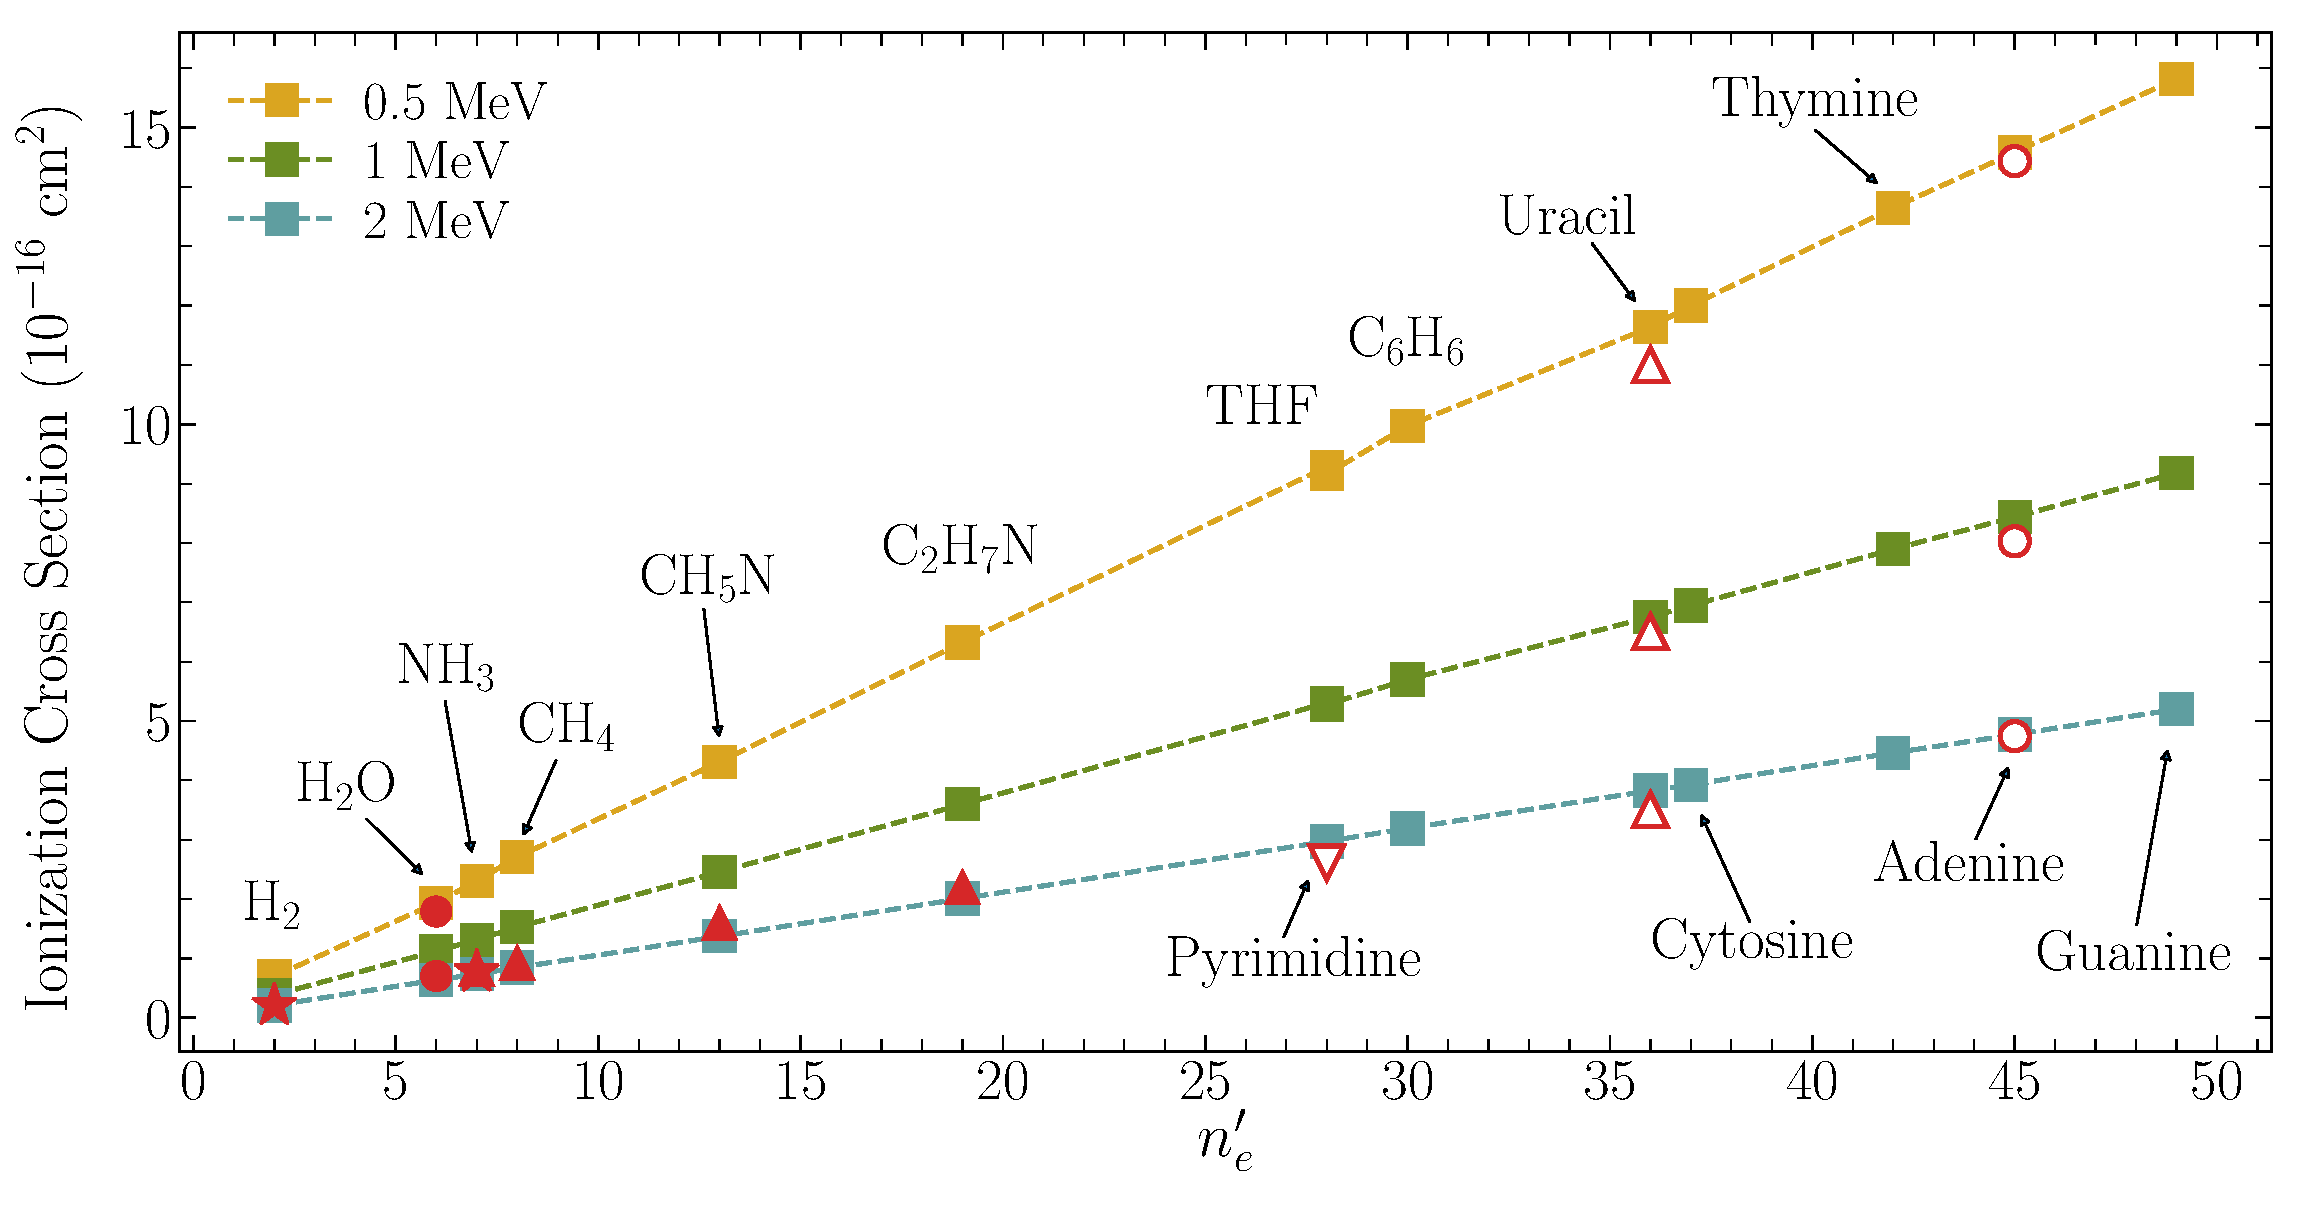
\includegraphics[width=0.9\textwidth]{ionmol/scale_ne.eps}
\caption[Ionización por impacto de protón en términos de $n_e'$.]
{Sección eficaz de ionización por impacto de protón a $0.5$, 1, y 2~MeV 
en términos del númbero de electrones activos dado por la 
Tabla~\ref{tab:ne_molecules}. Símbolos: 
\mbox{\Large$\circ$}~adenina~\cite{Iriki:11}, 
$\triangle$ uracilo~\cite{itoh2013}, 
$\bigtriangledown$ pirimidina~\cite{wolff2014}, 
$\blacktriangle$ C$_2$H$_7$N, CH$_5$N, metano y amoníaco~\cite{Lynch:76},
\mbox{\scriptsize$\bigstar$} amoníaco y H$_2$~\cite{Rudd:85}, y 
\mbox{\Large$\bullet$} agua~\cite{Luna2007}.}
\label{fig:recta}
\end{figure}

Podemos examinar de forma alternativa la escala definida por los números 
CDW dibujando las secciones eficaces de ionización de las moléculas en 
función de los valores dados para $n_e'$ según la 
Tabla~\ref{tab:ne_molecules} en ciertos valores de energía. Nuestros 
resultados se muestran en la Fig.~\ref{fig:recta} para energías de 
impacto de $0.5$, 1 y 2~MeV. Como puede observarse, las secciones 
eficaces de ionización CDW calculadas para todas las moléculas muestran 
una dependencia lineal con el número de electrones CDW $n_e'$ de la 
Tabla~\ref{tab:ne_molecules}. Obtenemos resultados similares, incluso 
para $E=10$~MeV. La comparación con los datos experimentales disponibles 
muestra una buena concordancia general, desde moléculas pequeñas, tales 
como H$_2$, CH$_4$ y NH$_3$, hasta las más complejas, como la adenina. 
Para los datos de ionización por impacto de electrón, los datos 
experimentales se interpolaron entre vecinos cercanos. 
%It is worth mentioning that an equivalent plot using the Toburen numbers 
%$n_e$ does not exhibit the straight lines obtained with the present scaling. 

%While finishing the present work, we became aware of an accepted 
%manuscript by L\"udde~\textit{et al.}~\cite{ludde2019} on total 
%ionization of biological molecules by proton impact, using the
%independent--atom--model pixel counting method~\cite{ludde2016,ludde2018}.
%The authors also raised a scaling  with $\nu_{\alpha}=4$ for C, N, and O. 
%The agreement with this independent method for proton impact reinforces 
%our multicharged--ion findings.

%%%%%%%%%%%%%%%%%%%%%%%%%%%%%%%%%%%%%%%%%%%%%%%%%%%%%%%%%%%%%%%%%%%%%%%%
\subsection{Escala con la carga del ion}
\label{sec:zscaling}
%%%%%%%%%%%%%%%%%%%%%%%%%%%%%%%%%%%%%%%%%%%%%%%%%%%%%%%%%%%%%%%%%%%%%%%%

A energías de impacto intermedias, la regla $Z^2$ no se cumple y se 
pueden considerar otras escalas en esta región. Encontramos en la 
literatura dos tipos de leyes de escala con la carga $Z$ del ion 
incidente aplicables en este rango de energías de impacto. La regla 
sugerida por Janev y Presnyakov~\cite{Janev:80} considera $\sigma/Z$ en 
función de $E/Z$ como la forma reducida \textit{natural} de la sección 
eficaz de ionización $\sigma$ y la energía de ion incidente $E$. Más 
recientemente, Montenegro y colaboradores~\cite{Dubois:13,Montenegro:13} 
sugirieron una expresión alternativa, la cual toma en cuenta que la 
sección eficaz es una función de $Z^2/E$ a altas energías. La escala 
propuesta, dada por
\begin{equation}
 \sigma/Z^{\alpha}=f(E/Z^{2-\alpha}),
\label{eq:Montenegro}
\end{equation}
mantiene la relación $Z^2/E$ para cualquier valor del parámetro $\alpha$. 
Los autores propusieron el valor $\alpha=4/3$ para la ionización de He y
H$_2$ debido al impacto de diversos iones cargados~\cite{Dubois:13}. 

Siguiendo el trabajo de Montenegro y colaboradores, optimizamos el 
parámetro~$\alpha$ de manera tal que los resultados obtenidos por la 
combinación del método CDW y SSM para los sistemas colisionales 
moleculares estudiados aquí convergan en el mayor rango de energías 
posible (de intermedias a altas). El resultado de dicha optimización es 
$\alpha=1.2$. La validez de este particular escaleo es evidente en la 
Fig.~\ref{fig:zreduced}, donde --para cada blanco-- las curvas SSM--CDW 
correspondientes a los diferentes iones se superponen. Es notable como 
los resultados teóricos son válidos para energías de impacto incluso por 
encima del máximo de las secciones eficaces, que corresponden a rangos de 
energías incidentes desde 50 keV para H$^+$ hasta 250 keV/amu para 
O$^{+8}$.

\begin{figure}
\centering
\includegraphics[width=0.9\textwidth]{ionmol/adn1_zscale.eps}
\caption[Sección eficaz de ionización reducida por $Z$ y $\alpha$ 
(Parte I).]
{Sección eficaz de ionización reducida $\sigma/Z^{\alpha}$ como función
de la energía incidente del ion $E/Z^{2-\alpha}$ con $\alpha=1.2$. 
Curvas: resultados teóricos CDW-SSM. 
Símbolos: datos experimentales de la Fig.~\ref{fig:crossDNA_1}.}
\label{fig:zreduced}
\end{figure} 

\begin{figure}
\centering
\includegraphics[width=0.9\textwidth]{ionmol/adn2_zscale.eps}
\caption[Sección eficaz de ionización reducida por $Z$ y $\alpha$ 
(Parte II).]
{Sección eficaz de ionización reducida $\sigma/Z^{\alpha}$ como función
de la energía incidente del ion $E/Z^{2-\alpha}$ con $\alpha=1.2$. 
Curvas: resultados teóricos CDW-SSM. 
Símbolos: datos experimentales de la Fig.~\ref{fig:crossDNA_2}.}
\label{fig:zreduced}
\end{figure} 

También examinamos los datos experimentales disponibles para los sistemas
ion-blanco bajo estudio~\cite{Iriki:11,Sens:20,Bhattacharjee:19,itoh2013,
wolff2014,wang2016,agnihotri2012,agnihotri2013,Luna2007,Bolorizadeh86,
H_Rudd85,He_Rudd85,toburen80,Ohsawa05,Bhattacharjee:17,DalCappello:09,
Bhattacharjee:16} con la regla de escala $Z^\alpha$. En el caso de los 
blancos con pocos o ningún dato experimental incluimos secciones eficaces 
experimentales de ionización por impacto de electrón~\cite{Rahman:16,
bug2017,wolf2019,fuss2009} a grandes velocidades con la conversión 
correspondiente. Como se observa, la mayor parte de los datos 
experimentales en la Fig.~\ref{fig:zreduced} confirma el escaleo sugerido 
aquí, incluso para O$^{+8}$ en agua~\cite{Bhattacharjee:16}. 

%%%%%%%%%%%%%%%%%%%%%%%%%%%%%%%%%%%%%%%%%%%%%%%%%%%%%%%%%%%%%%%%%%%%%%%%
\subsection{Escala con electrones activos y carga del ion}
\label{sec:nez_scaling}
%%%%%%%%%%%%%%%%%%%%%%%%%%%%%%%%%%%%%%%%%%%%%%%%%%%%%%%%%%%%%%%%%%%%%%%%

Considerando la reducción con la carga del ión incidente $Z^\alpha$ y el 
escaleo con el número de electrones activos del blanco, introducimos 
la sección eficaz de ionización molecular independiente $\tilde{\sigma}$, 
que se expresa como función de $\tilde{E}=E/Z^{2-\alpha}$, y está dada por
\begin{equation}
 \tilde{\sigma}\left(\tilde{E}\right)=\frac{\sigma_e}{Z^{\alpha}}
 =\frac{\sigma_M}{n_e'\,Z^{\alpha}}\,,
\label{eq:u-scaling}
\end{equation}
donde $\sigma_M$ es la sección eficaz de ionización de un blanco 
molecular, $n_e'$ es el número de electrones activos por molécula dado
en la Tabla~\ref{tab:ne_molecules}, y el parámetro es $\alpha=1.2$. La 
Fig.~\ref{fig:zalpha} muestra los valores teóricos y experimentales de 
$\tilde{\sigma}$ para todos los sistemas moleculares de la 
Tabla~\ref{tab:families}. Como se observa, la regla de escala combinada 
funciona muy bien y es independiente tanto de la naturaleza del ion 
incidente como de la complejidad del blanco molecular. Nuestros 
resultados teóricos SSM--CDW se ubican en una banda estrecha válida para 
cualquier ion incidente (reducida con $Z^\alpha$) en cualquier molécula
(escalada con el número de electrones activos $n_e'$) con una dispersión 
de aproximadamente $\pm 20\%$. Si consideramos los valores experimentales
disponibles, la incertidumbre de nuestra escala independiente crece a 
$\pm 30\%$, esquematizada en la Fig.~\ref{fig:zreduced} con un área gris. 
Notar que no hemos incluido en esta figura los resultados para uracilo de 
las Refs.~\cite{agnihotri2012,agnihotri2013}. 

\begin{figure}[t]
\centering
\includegraphics[width=0.9\textwidth]{ionmol/Zne_scaling.eps}
\caption[Sección eficaz de ionización reducida por $Z$ y $n_e$.]
{Sección eficaz de ionización reducida con la carga $Z$ del ion incidente
y escalada con el número de electrones activo $n_e$ del blanco molecular,
dado por la ecuación~(\ref{eq:u-scaling}) con $\alpha=1.2$. 
Curvas: resultados teóricos CDW-SSM. Símbolos: datos experimentales de 
las Figs.~\ref{fig:crossDNA_1} y \ref{fig:crossDNA_2}.}
\label{fig:zalpha}
\end{figure} 

Proponemos que la regla de escala independiente propuesta es válida para 
cualquier combinación ion--molécula. Para evaluar la generalidad de 
nuestro modelo, incluimos en la Fig.~\ref{fig:zreduced} un grupo de datos 
experimentales correspondientes a blancos moleculares no considerados en 
el diseño de esta regla, tales como las mediciones de 
Rudd~\textit{et al.}~\cite{Rudd:85,Rudd:83} para H$^{+}$ y He$^{+2}$ 
en N$_2$, O$_2$, CH$_4$, CO y CO$_2$, y los recientes experimentos de
Luna~\textit{et al.} \cite{Luna2019} de H$^{+}$ en CH$_4$. 

El buen acuerdo entre los resultados previstos por nuestro modelo y los
datos experimentales disponibles que se muestran en la 
Fig.~\ref{fig:zalpha} resume los principales resultados de esta 
investigación. Nuestro regla de escala independiente muestra ser eficaz 
no solo para predecir la ionización de los sistemas ion--blanco 
estudiados aquí sino también muestra potencial para reproducir una gran 
variedad de sistemas colisionales. Aunque los resultados teóricos 
SSM--CDW son válidos para energías por debajo del máximo de la sección 
eficaz de ionización, se puede observar en la Fig.~\ref{fig:zalpha} como 
el escaleo de los datos experimentales se extiene aún para valores de 
energía incidente menores. Esperamos que mediciones experimentales para 
otros iones y moléculas refuercen el modelo y escaleo propuesto.

%%%%%%%%%%%%%%%%%%%%%%%%%%%%%%%%%%%%%%%%%%%%%%%%%%%%%%%%%%%%%%%%%%%%%%%%
\section{Estructura molecular de los blancos}
\label{sec:molcalculations}
%%%%%%%%%%%%%%%%%%%%%%%%%%%%%%%%%%%%%%%%%%%%%%%%%%%%%%%%%%%%%%%%%%%%%%%%

Finalmente, para probar el rango de validez del SSM, realizamos un 
cálculo de estructura molecular de primeros principios para cinco 
nucleobases empleando el código {\sc gamess}. Los cálculos de energía de 
un centro se realizaron implementando el método restringido de 
Hartree--Fock con optimización de geometría y el conjunto de bases 
gaussianas 3-21G. 

\begin{figure}
\centering
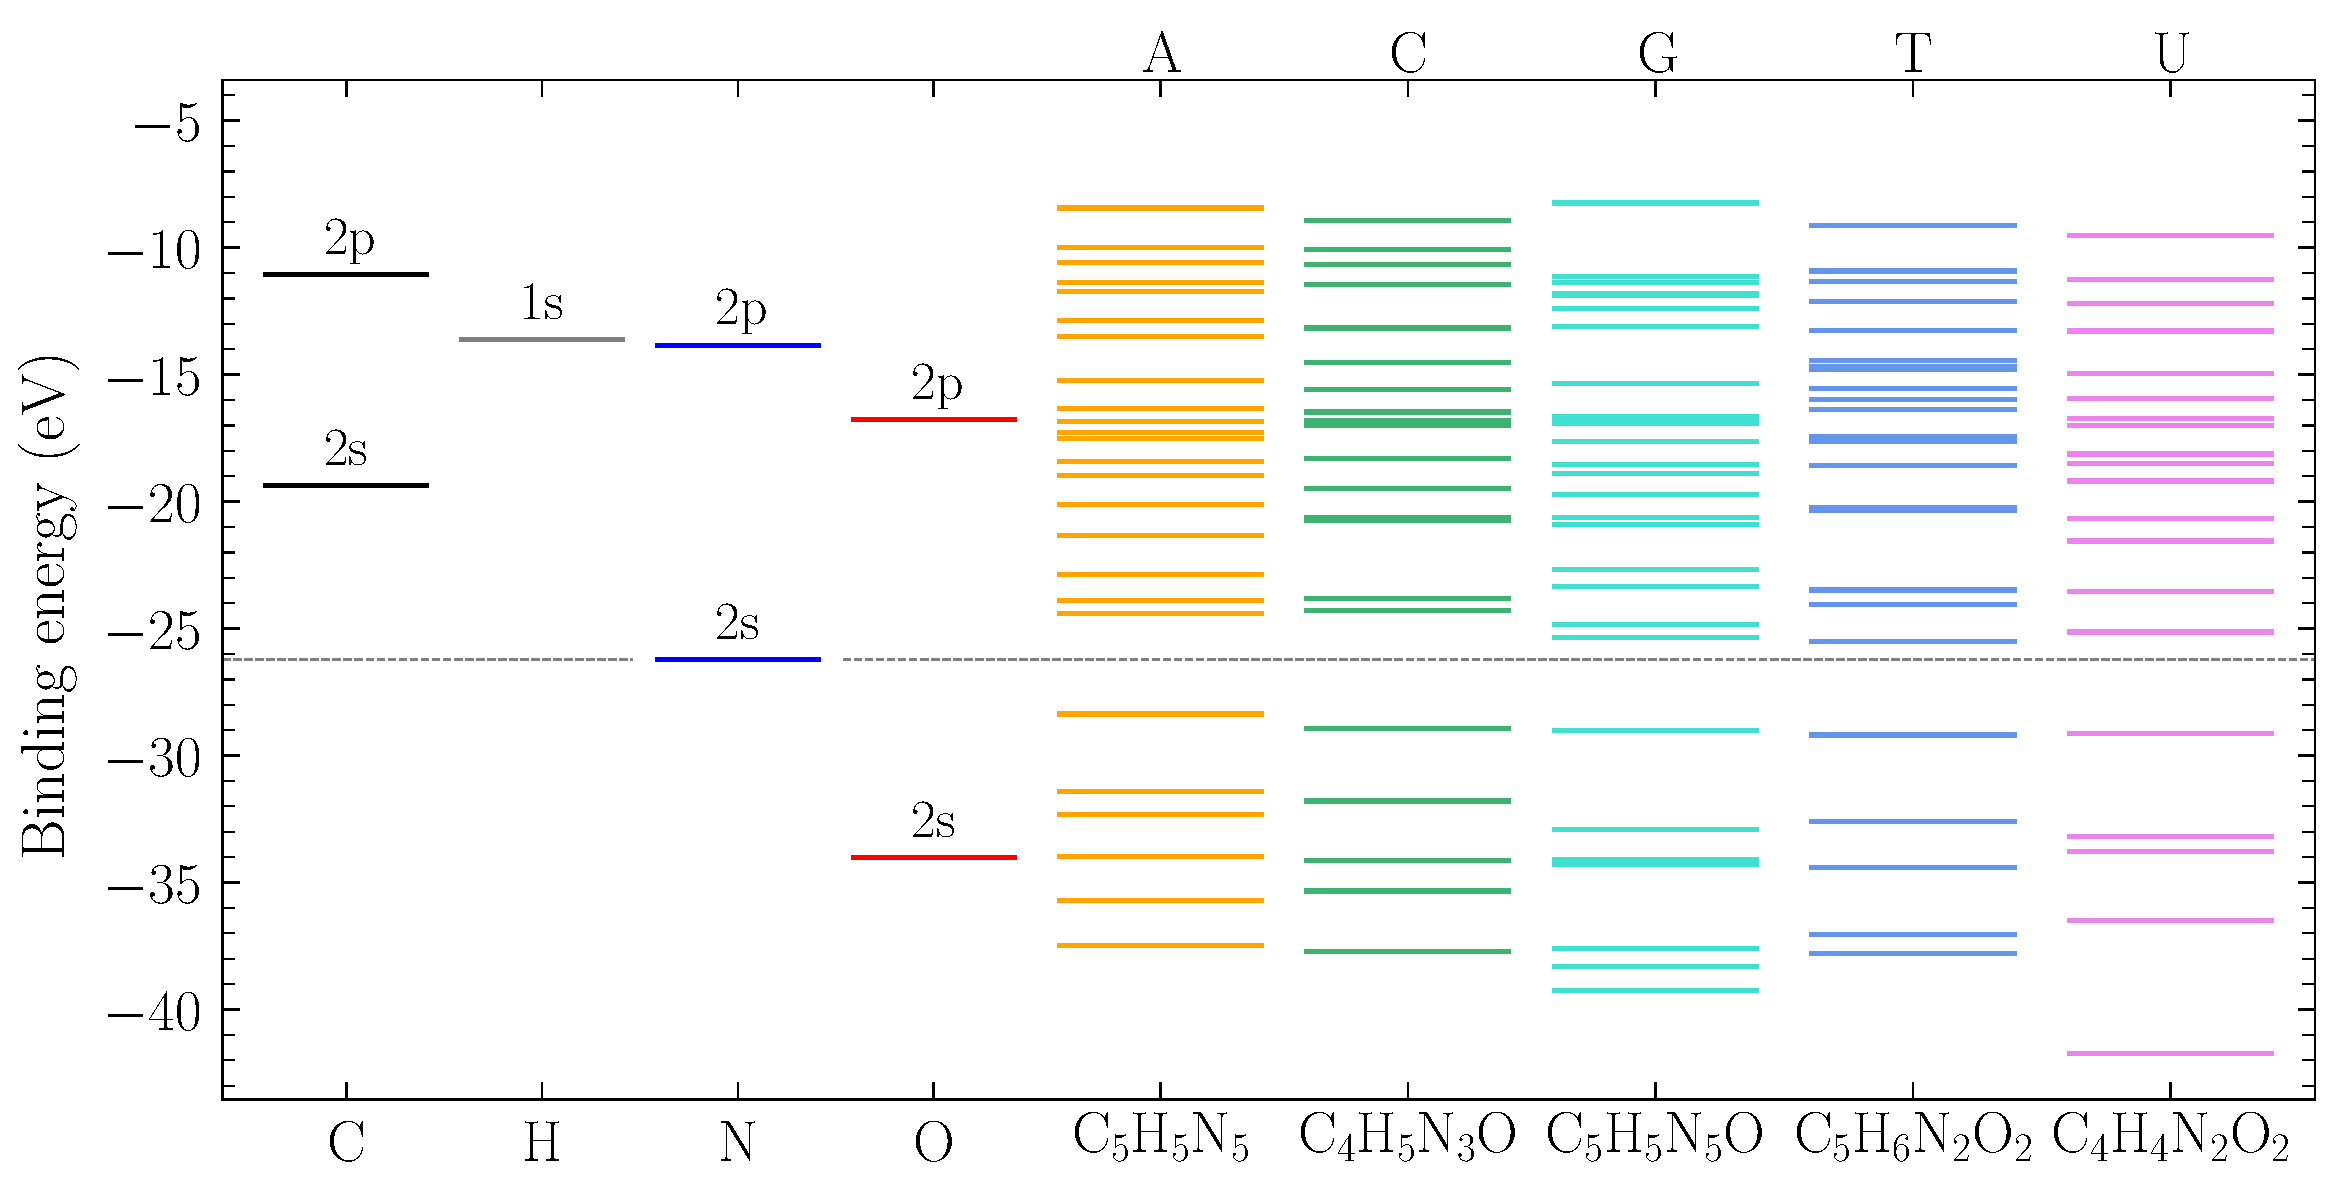
\includegraphics[width=0.9\textwidth]{ionmol/levelsDNA.eps}
\caption[Energías de ligadura moleculares teóricas de ADN y ARN.]
{Energías de ligadura moleculares teóricas de adenina, citosina, guanina, 
timina, y uracilo, comparado con los valores correspondientes de los 
átomos que las constituyen.}
\label{fig:bindener}
\end{figure}

En la Fig.~\ref{fig:bindener} se muestran las energías de ligadura 
molecular de los electrones de valencia para las nucleobases: adenina, 
citosina, guanina, timina y uracilo. Las energías de ligadura del orbital 
molecular más alto (HOMO) obtenidos concuerdan con los valores 
experimentales~\cite{Hush,Verkin,Dougherty} en un 2\% para todas las 
moléculas consideradas. En la izquierda de la Fig.~\ref{fig:bindener}, 
mostramos las energías atómicas de Hartree-Fock de los elementos 
constituyentes. Esta comparación nos da una idea de la distribución de 
los electrones débilmente ligados en las moléculas. Se traza una línea 
discontinua alrededor de $-26$~eV para separar la banda molecular en dos. 
Podemos considerar los niveles de energía atómica por encima de esta 
línea como los correspondientes a los electrones débilmente ligados de la 
Ec.~(\ref{eq:neCDW}). Por ejemplo, los electrones $2s$ y $2p$ del 
carbono se ubican por encima de la línea discontinua, que corresponde a 
los cuatro electrones dados por los números CDW. En el caso de O, solo 
los cuatro electrones de los orbitales 2p se encuentran por encima de la 
línea divisoria propuesta, que se corresponde con el número de electrones
débilmente ligados dado por el escaleo CDW. El caso del átomo de N no es 
tan directo; el número $\nu_{N}^{\text{CDW}}=4$ sugiere que sólo uno de 
los dos electrones de la capa $2s$ contribuye al esquema molecular.

%%%%%%%%%%%%%%%%%%%%%%%%%%%%%%%%%%%%%%%%%%%%%%%%%%%%%%%%%%%%%%%%%%%%%%%%
\subsection{Un modelo estequiométrico modificado}
%%%%%%%%%%%%%%%%%%%%%%%%%%%%%%%%%%%%%%%%%%%%%%%%%%%%%%%%%%%%%%%%%%%%%%%%

El modelo estequiométrico propuesto en la Sección~\ref{sec:SSM} considera 
a la molécula $M$ como un conjunto de átomos neutros aislados, lo cual es 
definitivamente irreal. Una primera mejora se puede sugerir asumiendo que 
los átomos no son efectivamente neutrales y que tienen una distribución 
dispar de los electrones dentro de la molécula. Esta característica puede 
expresarse mediante una carga efectiva $q_{\alpha}$ por átomo. La carga 
de Mulliken proporciona un valor posible para $q_{\alpha}$; sin embargo, 
existe una gran variedad de posibles distribuciones de 
carga~\cite{lee2003}.

\begin{table}
\begin{center}
\begin{tabular}{|p{0.12\textwidth}|p{0.08\textwidth}|p{0.08\textwidth}|p{
0.08\textwidth}|p{0.08\textwidth}|p{0.28\textwidth}|}
\hline
Molécula & C & H & N & O & Estequiometría de carga \\
\hline
Adenina & +0.32 & +0.23 & --0.55 &       & 
C$_{4.92}$H$_{4.77}$N$_{5.14}$ \\ 
\hline
Citosina & +0.28 & +0.21 & --0.56 & --0.53 & 
C$_{3.93}$H$_{4.79}$N$_{3.14}$O$_{1.13}$ \\ 
\hline
Guanina & +0.46 & +0.20 & --0.58 & --0.36 & 
C$_{4.89}$H$_{4.80}$N$_{5.15}$O$_{1.09}$ \\ 
\hline
Timina & +0.20 & +0.19 & --0.54 & --0.52 & 
C$_{4.95}$H$_{5.81}$N$_{2.13}$O$_{2.13}$ \\ 
\hline
Uracilo & +0.31 & +0.22 & --0.59 & --0.47 & 
C$_{3.92}$H$_{3.78}$N$_{2.15}$O$_{2.12}$ \\ 
\hline
\end{tabular}
\caption[Cargas efectivas medias de Mulliken por átomo]
{Cargas efectivas medias de Mulliken por átomo $q_{\alpha}$, y nueva formula
estequiométrica definida por la ecuación~(\ref{eq:newstoi}) para cinco
moléculas de ADN.}
\label{tab:newstoi}
\end{center}
\end{table}

Para tomar en cuenta este efecto, consideramos que el número total de 
electrones $Q_{\alpha }$ en el elemento $\alpha$ se distribuye de forma
dispar sobre todos los átomos $\alpha$. Por lo tanto, cada elemento  
$\alpha$ tendrá una carga $q_{\alpha}=Q_{\alpha}/n_{\alpha}$, que puede 
ser positiva o negativa. Este valor dependerá de la electronegatividad 
relativa respecto a los otros átomos~\cite{rappe1991}. Siguiendo esta 
idea, podemos estimar el número fraccional de átomos por molécula 
$n_{\alpha}'$, el cual está dado por 
\begin{equation}
n_{\alpha }^{\prime }=n_{\alpha }-
\frac{q_{\alpha }}{\nu_{\alpha }^{\text{CDW}}}
\label{eq:newstoi}
\end{equation}
En el caso de átomos neutrales, $q_{\alpha}=0$ y $n_{\alpha}'=n_{\alpha}$,
como dispone el SSM. En la Tabla~\ref{tab:newstoi}, mostramos un valor 
promedio de carga efectiva por átomo $q_{\alpha}$ de C, H, N, y O, para 
cinco moléculas del ADN, las cuales se obtuvieron a partir de los 
cálculos de estructura molecular descritos en la sección anterior.

Implementando la Ec.~(\ref{eq:newstoi}), es posible determinar una nueva 
fórmula estequiométrica de carga, la cual se da en la última columna de 
la Tabla~\ref{tab:newstoi}). Ahora, en vez de tener un número entero de 
átomos $n_{\alpha}$, tenemos un número fraccional dado por $n_{\alpha}'$. 
Se pueden calcular nuevas secciones eficaces moleculares, 
$\sigma'_{M}=\sum_{\alpha}n_{\alpha}'\sigma_{\alpha}$ considerando tales 
valores. Se calcularon errores relativos de las secciones eficaces de 
ionización para las bases de ADN de la Tabla~\ref{tab:newstoi}. Las 
diferencias obtenidas fueron menores de 3\%, lo cual indica que el modelo 
estequiométrico es un modelo robusto con el que se pueden modelar este 
tipo de moléculas complejas dentro del margen de error esperado.

%%%%%%%%%%%%%%%%%%%%%%%%%%%%%%%%%%%%%%%%%%%%%%%%%%%%%%%%%%%%%%%%%%%%%%%%
\section{Conclusiones}
%%%%%%%%%%%%%%%%%%%%%%%%%%%%%%%%%%%%%%%%%%%%%%%%%%%%%%%%%%%%%%%%%%%%%%%%

En este capítulo, hemos estudiado la ionización de blancos moleculares 
de interés biológico debido al impacto de iones de carga múltple. Se han
calculado secciones eficaces de ionización de gran número de blancos 
moleculares de interés biologico conteniendo H, C, N y O por el impacto 
de antiprotones, H$^{+}$, He$^{2+}$, Be$^{4+}$, C$^{6+}$, y O$^{8+}$. 
Nuestras prediciones teóricas han sido obtenidas combinando la 
implementación del método de onda continua distorsionada con estado 
inicial de Eikonal para blancos atómicos (descritos con potenciales 
efectivos DIM), para modelar el proceso colisional, y el modelo 
estequiométrico simple, para aproximar la estructura de las moléculas. 
Presentamos secciones eficaces de ionización total para adenina, 
citosina, timina, guanina, uracilo, THF y agua, siendo comparadas a su 
vez con datos experimentales disponibles. 

Estudiamos y calcularon valores medios de energía y ángulo de emisión de 
los electrones ionizados de blancos atómicos, que son de importancia en 
el daño secundario de las colisiones con iones. Nuestros resultados 
muestran una clara dependencia de estos valores con la carga del ion $Z$. 
Para un blanco dado, a medida que $Z$ aumenta, $\overline{E}_{\alpha}$ 
también aumentan. Por otro lado, $\overline{\theta}_{\alpha}$ decrece, lo 
que muestra una clara tendencia a la dirección del ion. A energía de 
impacto mayores a 2~MeV/amu, estos valores convergen a la primera 
aproximación de Born, la cual establece la simple ley de escala $Z^{2}$. 

Propusimos tres reglas de escala para las secciones eficaces de 
ionización para blancos de interés biológico por cuatro iones desnudos. 
Primero, exploramos la ampliamente usada regla de escala de Toburen, que 
escala la sección eficaz de ionización molecular con un determinado 
número de electrones débilmente ligados. Luego, a partir de los 
resultados CDW para los atómos H, C, N y O, encontramos que la respuesta 
de las secciones eficaces de ionización puede ser optimizada 
normalizándolas con diferentes números de electrones activos en la 
colisión. Así, definimos la primera regla de escala con el número de 
electrones activos CDW, la cual provee buenos resultados para los 
sistemas proyectil--molécula estudiados aquí. La comparación con los 
datos experimentales refuerza nuestros hallazgos. Además, probamos la 
regla de escala CDW mediante la inclusión de datos experimentales de 
ionización de H$_2$, metano y amoníaco por impacto de protones, los 
cuales muestran una buena concordancia en el rango de energías 
intermedias a altas. La segunda regla de escala propuesta considera el 
ion incidente, reduciendo la naturaleza del proyectil mediante el escaleo 
de la sección eficaz de ionización con la carga del ión, $Z^{\alpha}$, 
como una función de la energía incidente reducida $E/Z^{2-\alpha}$, 
siendo $\alpha=1.2$. La última regla que proponemos combina el escaleo de 
la sección eficaz de ionización total con el número de electrones activos 
CDW y la reducción con la carga del ión, $Z^{\alpha}$, lo cual conduce a 
una ley de escala independiente de la carga del ion y el blanco 
molecular. Las tres reglas de escala obtenidas mediante nuestro modelo 
SSM--CDW para los 80 sistemas colisionales examinados fueron comparadas 
con datos experimentales disponibles. Luego, la generalidad de nuestra 
regla de escala independiente fue inspeccionada mediante la inspección
de un número significativo de datos experimentales para otros sistemas 
colisionales (no considerados previamente), probando ésta ser válida 
incluso para energías fuera del rango de validez del método SSM--CDW.

Finalmente, realizamos cálculos de estructura molecular para las 
nucleobases del ADN. Al inspeccionar las energías de ligadura moleculares 
obtenidas mediante cálculos mecanicocuánticos de primeros principios, 
pudimos comprender el número de electrones resultantes de la optimización 
basada en los cálculos CDW. Intentamos mejorar el modelo estequiométrico 
utilizando la carga de Mulliken para obtener proporciones fraccionarias 
en lugar de enteras para el número de átomos constituyentes. No 
encontramos una corrección sustancial, lo que indica que el SSM funciona 
bastante bien. Los presentes resultados refuerzan la exactitud del modelo 
estequiométrico simple y la aproximación CDW para tratar la ionización de 
moléculas complejas por el impacto de iones cargados en el rango de 
energía intermedia a alta. 

